\documentclass[border=6pt]{standalone}
\usepackage[T1]{fontenc}
\usepackage{lmodern}
\usepackage{amsmath,amssymb,bm}
\usepackage{xcolor}
\usepackage{tikz}
\usetikzlibrary{arrows.meta,positioning,fit,backgrounds,calc}
\definecolor{swinc}{HTML}{2166AC}
\definecolor{cnnc}{HTML}{1B7837}
\definecolor{decc}{HTML}{E66101}
\definecolor{botc}{HTML}{B2182B}
\definecolor{headc}{HTML}{762A83}
\newcommand{\code}[1]{\texttt{\detokenize{#1}}}
\begin{document}
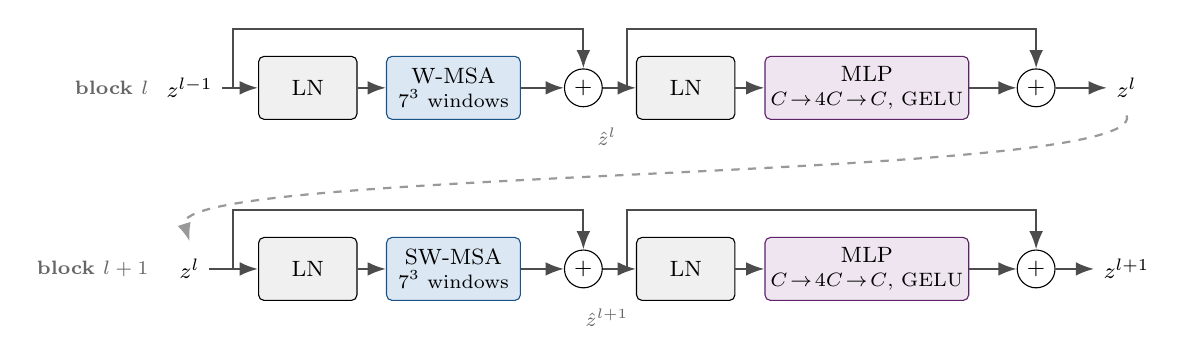
\begin{tikzpicture}[
  font=\footnotesize, >=Latex,
  op/.style={draw, rounded corners=2pt, minimum height=0.8cm, minimum width=1.25cm, align=center, inner sep=2pt},
  ln/.style={op, fill=black!6},
  msa/.style={op, fill=swinc!16, draw=swinc!80!black, minimum width=1.7cm},
  mlp/.style={op, fill=headc!12, draw=headc!80!black, minimum width=1.9cm},
  add/.style={draw, circle, inner sep=0pt, minimum size=0.48cm, fill=white},
  arr/.style={->, thick, black!70}
]
\foreach \row/\att/\zin/\zmid/\zout in {0/W-MSA/{z^{l-1}}/{\hat z^{l}}/{z^{l}}, -2.3/SW-MSA/{z^{l}}/{\hat z^{l+1}}/{z^{l+1}}} {
  \begin{scope}[yshift=\row cm]
    \node (i) at (0,0) {$\zin$};
    \node[ln] (n1) at (1.5,0) {LN};
    \node[msa] (a) at (3.35,0) {\att\\[-1pt]{\scriptsize $7^3$ windows}};
    \node[add] (p1) at (5.0,0) {$+$};
    \node[ln] (n2) at (6.3,0) {LN};
    \node[mlp] (m) at (8.6,0) {MLP\\[-1pt]{\scriptsize $C\!\to\!4C\!\to\!C$, GELU}};
    \node[add] (p2) at (10.75,0) {$+$};
    \node (o) at (11.9,0) {$\zout$};
    \draw[arr] (i) -- (n1); \draw[arr] (n1) -- (a); \draw[arr] (a) -- (p1);
    \draw[arr] (p1) -- (n2); \draw[arr] (n2) -- (m); \draw[arr] (m) -- (p2); \draw[arr] (p2) -- (o);
    \draw[arr] (0.55,0) -- (0.55,0.75) -| (p1.north);
    \draw[arr] (5.55,0) -- (5.55,0.75) -| (p2.north);
    \node[font=\scriptsize, text=black!60] at (5.3,-0.62) {$\zmid$};
  \end{scope}
}
\node[font=\scriptsize\bfseries, anchor=east, text=black!60] at (-0.4,0) {block $l$};
\node[font=\scriptsize\bfseries, anchor=east, text=black!60] at (-0.4,-2.3) {block $l+1$};
\draw[->, thick, black!40, dashed] (11.9,-0.35) .. controls (12.2,-1.2) and (-0.3,-1.0) .. (0,-1.95);
\end{tikzpicture}
\end{document}
